\section{Question Comme Document}
\subsection{Représentation et similarité de la question paddées/pertubée}
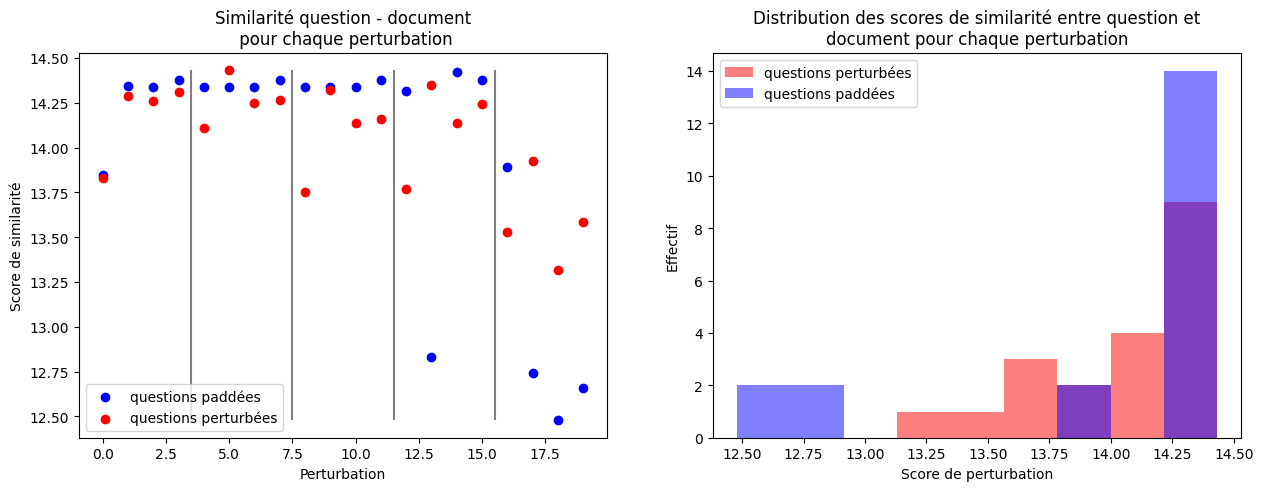
\includegraphics[width=\textwidth]{images/ScoresSimilarité_QuestionCommeDocument.png}



\paragraph{Dataset manipulé} 
Une paire (question, question) où la question est exploitée comme question mais aussi comme document

\paragraph{Perturbations appliquées}
\begin{verbatim}
drone -> engin autonome
limitation -> contrainte
système -> dispositif
technique -> spécialisé
drone -> vecteur
limitation -> bornage
système -> ensemble
technique -> difficile
drone->gazon
limitation->animation
système->panneau
technique->magique
drone->ver de verre
limitation->plastique anarchique
système->esperluette en vent
technique->feuille entubée
Full-replace Synonymes 1
         drone -> engin autonome
         limitation -> contrainte
         système -> dispositif
         technique -> spécialisé
Full-replace Polysémie 1
         drone -> vecteur
         limitation -> bornage
         système -> ensemble
         technique -> difficile
Full-replace Elephants 1
         drone -> gazon
         limitation -> animation
         système -> panneau
         technique -> magique
Full-replace Elephants Roses 1
         drone -> ver de verre
         limitation -> plastique anarchique
         système -> esperluette en vent
         technique -> feuille entubée
\end{verbatim}

\paragraph{Données représentées}
Le graphique de gauche représente les scores de pertinence de la question comme document pour chaque perturbation. Les questions non modifiées (représentées en bleu) sont juste paddées pour faire correspondre la taille du document non modifié avec celui perturbé (ici de la question perturbée, représentées en rouge). Les scores de pertinence pour chaque perturbation sont dans l'ordre des perturbations citées. Les lignes verticales séparent les perturbations par niveau (de 1 à 4 en allant de gauche à droite) puis regroupent les pertuabtion de type full\_replace (le plus à droite, de niveau 1 à 4 en allant de gauche à droite) 
Le graphique de droite est un histogramme des scores (en bleu pour la question paddée et en rouge pour la question perturbée)

\paragraph{Commentaires} 
On observe bien la différence de représentation entre les questions et les question perturbées. On constate aussi que le système de padding is en place par \cite{parry_mechir_2025} provoque une perturbation des documents. Certaines perturbations améliorent la similarité de la question avec elle même. Cela est surprenant



\subsection{Différence des scores de petinence pour question paddée et question perturbée}
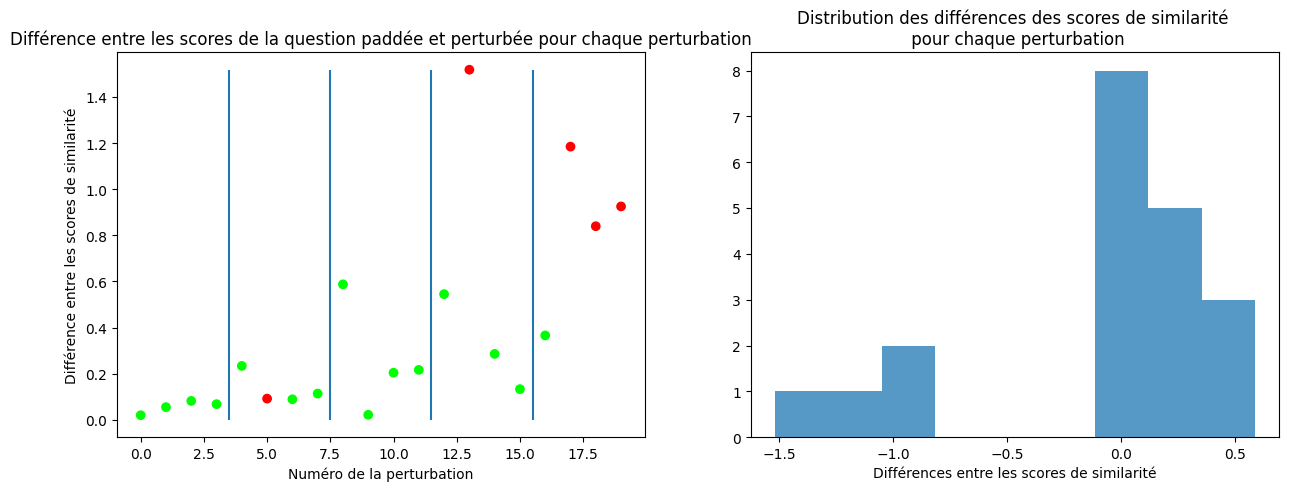
\includegraphics[width=\textwidth]{images/DifferencesScoresSimilarité_QuestionCommeDocument.png}

\paragraph{Données et perturbation}
Question comme document\\
Perturbation présentées précédemment

\paragraph{Lecture des graphiques}
Le graphique de gauche associe à chaque perturbation (dans l'ordre cité) la différence entre les scores de similarité à la question de la question perturbée et la question paddée pour la perturbation. Les points en rouge correspondnet à aux différences négatives et les points en vert aux différences positives. On attend des scores positifs car perturber un objet (en l'occurrence une question) réduit sa similarité à lui même. Les pints sont séparés pour identifier les pertubations de type replace de diférent niveau (1 à 4 de gauche à droite). Le cinquième (dernier) groupe correspond aux pertuabtions de type full\_replace (niveau 1 à 4 de gauche à droite)\\
Le grphique de droite représente la distribution de ces différences.

\paragraph{Analyse des graphiques}
Pour le premier graphique, on constate une augmentation de da différence pour les niveau les plus élevés concernnat les pertubations de type replace. Les perturbation de type full\_replace ont un effet de perturbation moins important que le padding induit par le modèle.